%!TEX root = ../documentation.tex
\chapter{Datenvorverarbeitung}
\label{ch:data_preprocessing}

\section{Bilddaten}

In der vorherigen Datenanalyse des Datensatzes wurden folgende Probleme herausgestellt:

\begin{enumerate}
	\item{Dimensionsunterschiede}
	\item{Farbunterschiede}
	\item{Kontrastunterschiede}
\end{enumerate}

Diese sollen nun mit geeigneten Vorverarbeitungsschritten gelöst werden.\\
Die Bilder müssen als Eingabe für das Model in einer einheitlichen Größe vorliegen. Dazu skalieren wir alle Bilder auf den Schwerpunkt der Dimensionen, welcher bei 320 x 320 Pixeln liegt.
Nur drei der Bilder sind kleiner als 320 x 320 Pixel und mussen damit vergrößert werden um die gewünschte Dimension zu erreichen. Bei einer Vergrößerung können Artifakte im Bild auftreten, welche das Training der Modelle negativ beeinflussen können. Aufgrund der geringen Anzahl können diese in unserer Datenlage vernachlässigt werden.\\
Farbliche Informationen spielen in den Röntgenbildern keine Rolle. Daher verwerfen wir die Farbinformationen und wandeln alle Farbbilder in Schwarzweißbilder um.\\
Weiterhin werden die Kontrastunterschiede über einen Histogrammausgleich verringert. Dadurch werden die Bilder, welche aus unterschiedlichen Quellen mit heterogenen Eigenschaften stammen, homogenisiert.

\pagebreak

Die Gesamtheit der Änderungen wird mithilfe der folgenden Beispielbilder verdeutlicht.

\begin{figure}[H]
	\centering
	\begin{subfigure}[t]{0.45\textwidth}
		\centering
		\includegraphics[width=\textwidth]{../images/42081.jpg}
		\caption{Originalbild 42081.jpg\\1524 x 1516 Pixel}
	\end{subfigure} \hfill
	\begin{subfigure}[t]{0.45\textwidth}
		\centering
		\includegraphics[width=\textwidth]{../train_data/42081.jpg}
		\caption{Vorverarbeitetes Bild\\320 x 320 Pixel}
	\end{subfigure} \hfill
	\caption{Vergleich eines Originalbildes mit dem daraus resultierenden vorverarbeiten Bild}
\end{figure}

\section{Datenaugmentation}

Bezüglich der Klassen haben wir in der zweiten Konstellation (zusammengefasste Krankheiten) eine ungleiche Verteilung festgestellt. Eine soche Ungleichverteilung beeinflusst dies die Leistung des Models in negativer Weise \cite{BUDA2018249}.\\
Um dieses Problem zu umgehen führen wir eine Offline-Datenaugmentation durch. Ein ähnlicher Ansatz wurde bereits in anderen Arbeiten \cite{UCAR2020109761} angewandt. Dabei werden aus einem Quellbild durch Transformationen mehrere zusätzliche Bilder erstellt. Diese werden dann in einem Verzeichnis auf der Festplatte abgelegt (offline).\\
Die Vorteile der Offline-Augmentation gegenüber einer Transformation während des Trainings der Modelle beläuft sich hauptsächlich auf eine geringere benötigte Rechenleistung. Ein einmal vorverarbeiteter Datensatz kann für mehrere Trainingsprozesse wiederverwendet werden.
Somit werden beispielsweise mehrere Iterationen während eines Hyperparameter-Tunings performanter.

\pagebreak

Zur Durchführung der beschriebenen Augmentation haben wir zunächst die folgenden Basistransformationen definiert.
Wichtig dabei ist, dass die strukturellen Informationen, welche die Krankheiten voneinander unterscheiden erhalten bleiben.
\begin{enumerate}[noitemsep]
	\item{Vertikale Spiegelung (Flip)}
	\item{Aufhellen (Bright)}
	\item{Verdunkeln (Dark)}
	\item{Gaußsche Unschärfe (Noise)}
	\item{Scherung (Shear)}
	\item{Rotation (Rotation)}
\end{enumerate}
Um die Anzahl der Transformationen weiter zu erhöhen und damit möglichst viele unterschiedliche Bilder zu erzeugen, haben wir weiterhin bis zu vier Basistransformationen geschachtelt.
Mit den daraus entstehenden zusammengesezten Transformationen erhalten wir insgesamt 20 Transformationen.

\begin{enumerate}[noitemsep]
	\item{Rotation + Aufhellen}
	\item{Spiegelung + Verdunkeln}
	\item{Spiegelung + Scherung}
	\item{Spiegelung + Rotation}
	\item{Scherung + Gaußsche Unschärfe}
	\item{Rotation + Scherung}
	\item{Gaußsche Unschärfe + Rotation}
	\item{Rotation + Aufhellen + Scherung}
	\item{Spiegelung + Scherung + Rotation}
	\item{Spiegelung + Scherung + Gaußsche Unschärfe}
	\item{Scherung + Rotation + Verdunkeln}
	\item{Gaußsche Unschärfe + Aufhellen + Scherung}
	\item{Spiegelung + Verdunkeln + Gaußsche Unschärfe}
	\item{Spiegelung + Rotation + Aufhellen + Scherung}
\end{enumerate}

Alle genannten Transformationen werden in Abbildung \ref{fig:augmentation} auf Seite \pageref{fig:augmentation} anhand eines Beispiels visualisiert.

\begin{figure}[H]
	\centering
	\begin{subfigure}[t]{0.2\textwidth}
		\includegraphics[width=\textwidth]{../train_data/18121.png}
		\caption{Vorverarbeitetes Bild}
	\end{subfigure} \hfill
	\begin{subfigure}[t]{0.2\textwidth}
		\includegraphics[width=\textwidth]{../aug_data/Augbright_18121.png}
		\caption{Bright}
	\end{subfigure} \hfill
	\begin{subfigure}[t]{0.2\textwidth}
		\includegraphics[width=\textwidth]{../aug_data/Augdark_18121.png}
		\caption{Dark}
	\end{subfigure} \hfill
	\begin{subfigure}[t]{0.2\textwidth}
		\includegraphics[width=\textwidth]{../aug_data/Augnoise_18121.png}
		\caption{Noise}
	\end{subfigure} \hfill
	\begin{subfigure}[t]{0.2\textwidth}
		\includegraphics[width=\textwidth]{../aug_data/Augflip_18121.png}
		\caption{Flip}
	\end{subfigure} \hfill
	\begin{subfigure}[t]{0.2\textwidth}
		\includegraphics[width=\textwidth]{../aug_data/Augrotation_18121.png}
		\caption{Rotation}
	\end{subfigure} \hfill
	\begin{subfigure}[t]{0.2\textwidth}
		\includegraphics[width=\textwidth]{../aug_data/Augshear_18121.png}
		\caption{Shear}
	\end{subfigure} \hfill
	\begin{subfigure}[t]{0.2\textwidth}
		\includegraphics[width=\textwidth]{../aug_data/Augflip_dark_18121.png}
		\caption{Flip + Dark}
	\end{subfigure} \hfill
	\begin{subfigure}[t]{0.2\textwidth}
		\includegraphics[width=\textwidth]{../aug_data/Augflip_dark_noise_18121.png}
		\caption{Flip + Dark + Noise}
	\end{subfigure} \hfill
	\begin{subfigure}[t]{0.2\textwidth}
		\includegraphics[width=\textwidth]{../aug_data/Augflip_rotation_18121.png}
		\caption{Flip + Rotation}
	\end{subfigure} \hfill
	\begin{subfigure}[t]{0.2\textwidth}
		\includegraphics[width=\textwidth]{../aug_data/Augflip_rotation_bright_shear_18121.png}
		\caption{Flip + Rotation + Bright + Shear}
	\end{subfigure} \hfill
	\begin{subfigure}[t]{0.2\textwidth}
		\includegraphics[width=\textwidth]{../aug_data/Augflip_shear_18121.png}
		\caption{Flip + Shear}
	\end{subfigure} \hfill
	\begin{subfigure}[t]{0.2\textwidth}
		\includegraphics[width=\textwidth]{../aug_data/Augflip_shear_noise_18121.png}
		\caption{Flip + Shear + Noise}
	\end{subfigure} \hfill
	\begin{subfigure}[t]{0.2\textwidth}
		\includegraphics[width=\textwidth]{../aug_data/Augflip_shear_rotation_18121.png}
		\caption{Flip + Shear + Rotation}
	\end{subfigure} \hfill
	\begin{subfigure}[t]{0.2\textwidth}
		\includegraphics[width=\textwidth]{../aug_data/Augnoise_bright_shear_18121.png}
		\caption{Noise + Bright + Shear}
	\end{subfigure} \hfill
	\begin{subfigure}[t]{0.2\textwidth}
		\includegraphics[width=\textwidth]{../aug_data/Augnoise_rotation_18121.png}
		\caption{Noise + Rotation}
	\end{subfigure} \hfill
	\begin{subfigure}[t]{0.2\textwidth}
		\includegraphics[width=\textwidth]{../aug_data/Augrotation_bright_18121.png}
		\caption{Rotation + Bright}
	\end{subfigure} \hfill
	\begin{subfigure}[t]{0.2\textwidth}
		\includegraphics[width=\textwidth]{../aug_data/Augrotation_bright_shear_18121.png}
		\caption{Rotation + Bright + Shear}
	\end{subfigure} \hfill
	\begin{subfigure}[t]{0.2\textwidth}
		\includegraphics[width=\textwidth]{../aug_data/Augrotation_shear_18121.png}
		\caption{Rotation + Shear}
	\end{subfigure} \hfill
	\begin{subfigure}[t]{0.2\textwidth}
		\includegraphics[width=\textwidth]{../aug_data/Augshear_noise_18121.png}
		\caption{Shear + Noise}
	\end{subfigure} \hfill
	\begin{subfigure}[t]{0.2\textwidth}
		\includegraphics[width=\textwidth]{../aug_data/Augshear_rotation_dark_18121.png}
		\caption{Shear + Rotation + Dark}
	\end{subfigure} \hfill
	\caption{Datenaugmentation dargestellt an einem Beispielbild}
	\label{fig:augmentation}
\end{figure}

Durch die Datenaugmentation kann das Ungleichgewicht bei der Verteilung der Klassen komplett aufgehoben werden, wie von der folgenden Abbildung dargestellt wird.
Dabei werden aus den möglichen 20 tranformierten Bildern einige randomisiert ausgewählt.
In der ersten Konstellation kann die Anzahl der COVID-19 Bilder an die Anzahl der Bilder ohne Befund angeglichen werden. Durch diese zusätzlichen Daten kann das gelernte Modell die beiden Klassen potentiell einfacher unterscheiden.

\begin{figure}[H]
	\centering
	\settowidth{\imagewidth}{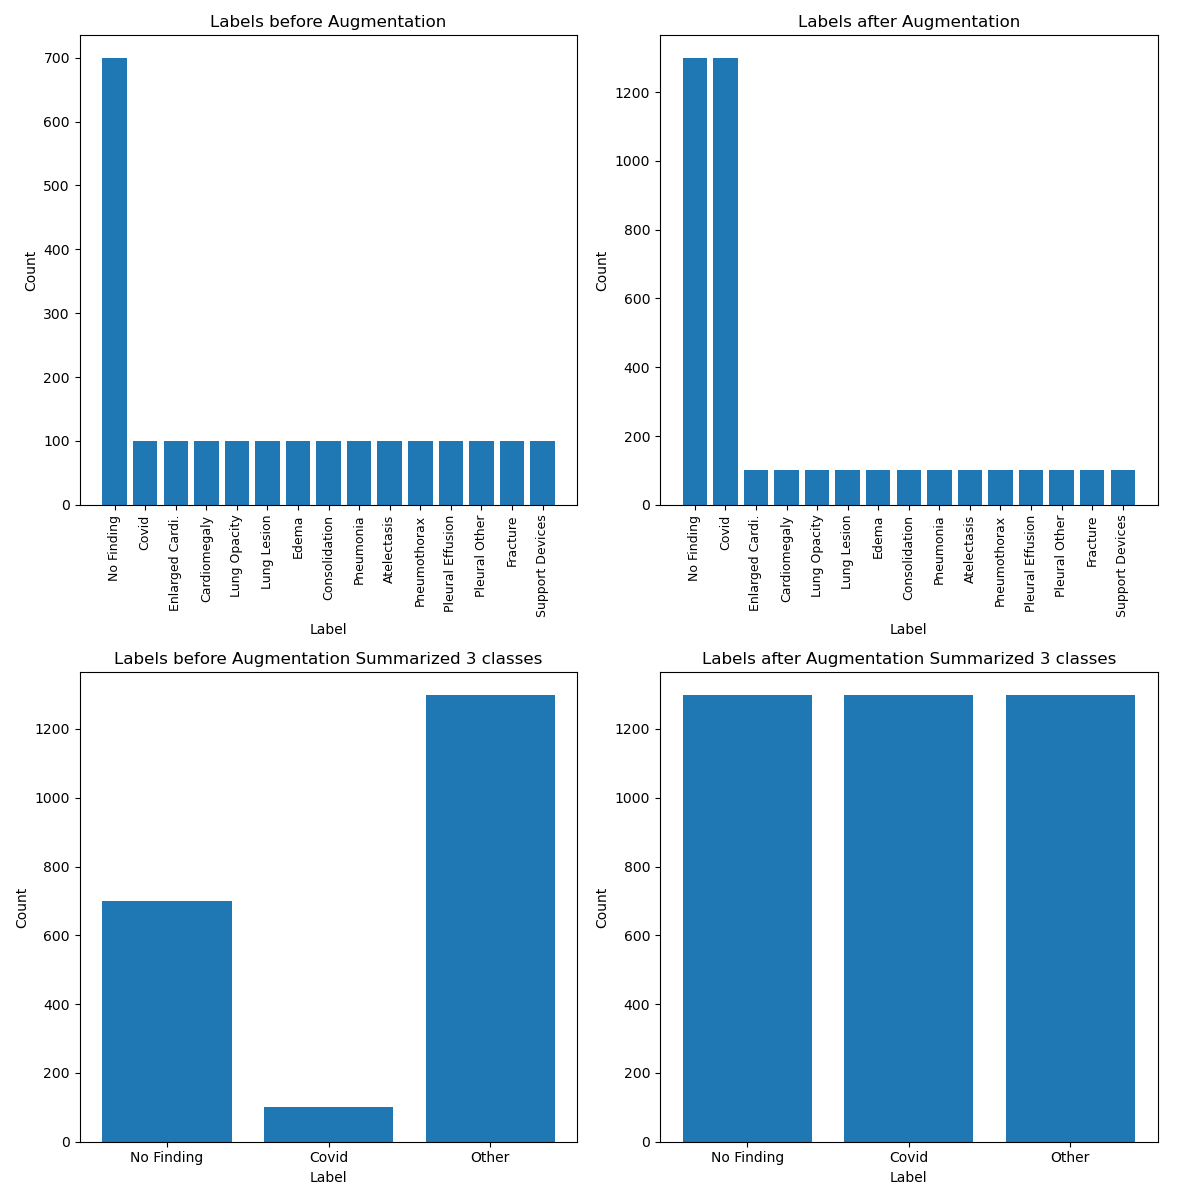
\includegraphics{../results/balancing.png}}
	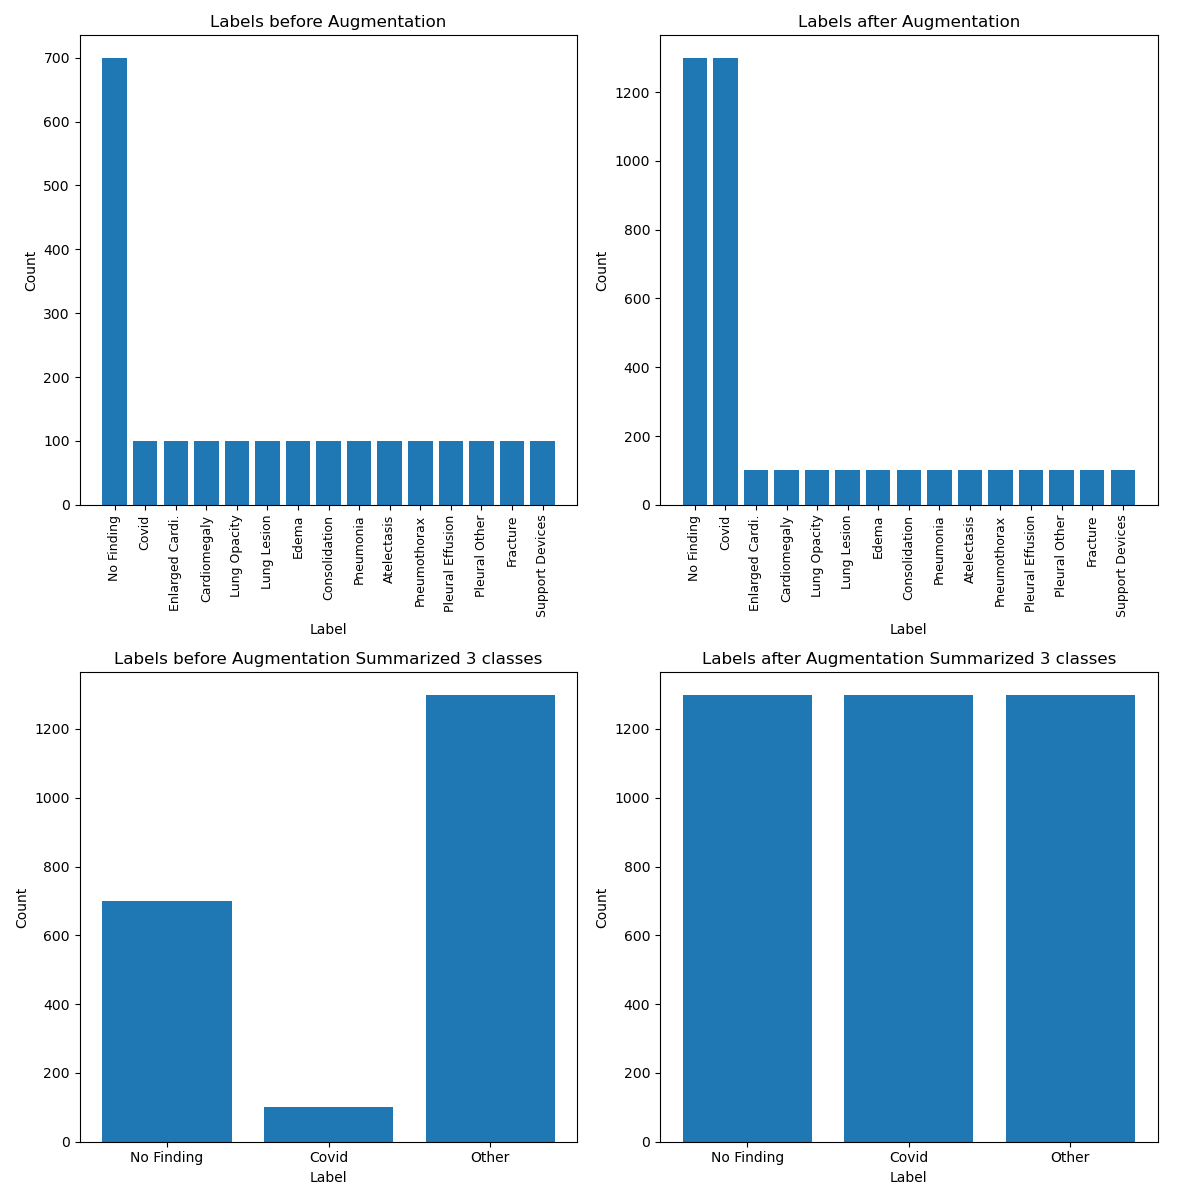
\includegraphics[trim=0.5\imagewidth{} 0 0 0, clip,width=0.275\imagewidth{}]{../results/balancing.png}
	\caption{Verteilung der Klassen nach Datenaugmentation}
	\label{fig:balancing}
\end{figure}

\section{Implementierung}

Zur Vorverarbeitung der Bilddaten und der Datenaugmentation dient das Python-Script \verb|preprocess.py|. Dessen Verwendung wird im Folgenden kurz beschrieben.

\begin{verbatim}
python preprocessing/preprocess.py [-h] [dataset] [output] [figure_output]
\end{verbatim}

Das \verb|dataset| Argument gibt analog zu den anderen Scripten das Verzeichnis an unter dem der Datensatz zu finden ist. Zusätzlich können über \verb|output| und \verb|figure_output| die Ausgabeverzeichnisse für die erzeugten Bilder und Grafiken bestimmt werden.\\
Es steht eine Programmhilfe über den optionalen Parameter \verb|-h| zur Verfügung.
